\section{Convolutional Neural Network}
\subsection{Vectorized convolution by Im2col and col2im}
The convolution operation can be implemented by many loops because the kernel will travel over the image. In terms of complexity, this is the easiest way to program but regard to timing, this idea is not efficient since it can only perform a convolution calculation sequentially. Now, with the highly support of hardward (explicitly GPU) that allows us to accelerate even more with parallel computation. In this part, we would like to break down 2 approaches in order to analyse their advantages and downsides.

\begin{figure}[H]
    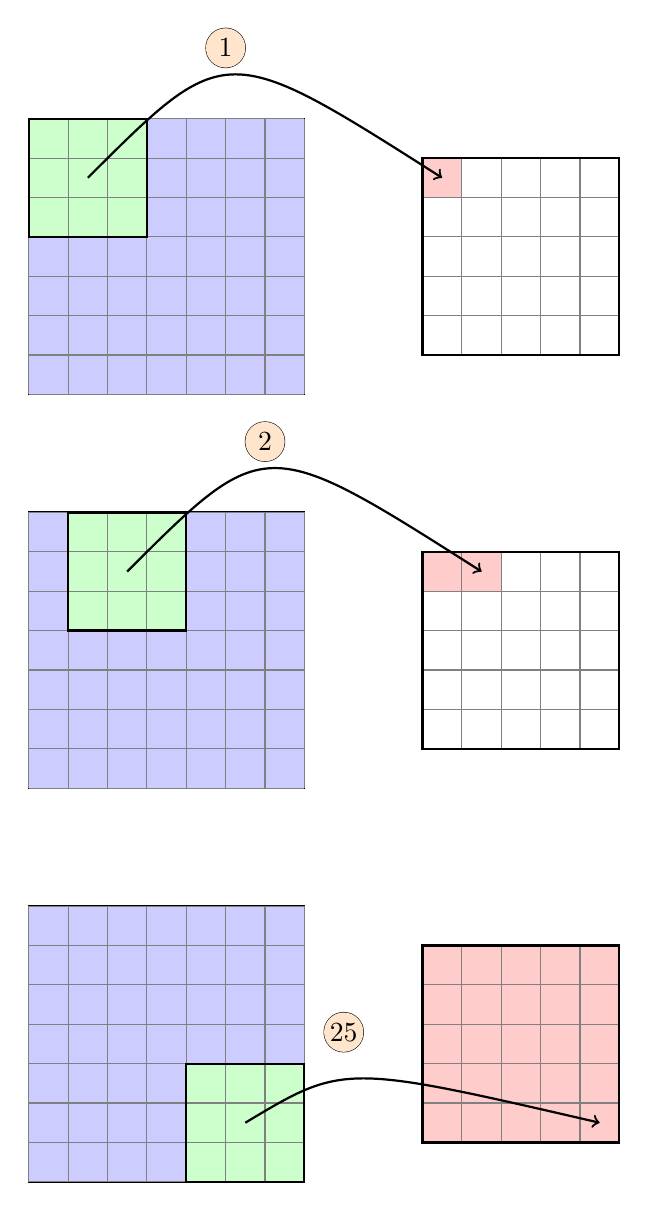
\begin{tikzpicture}
        \begin{scope}[scale=0.5]
            % Draw input convolution
            % Draw the outer rectangle border
            \draw[thick] (0,0) rectangle (7,7);
            
            % Fill the entire 7x7 grid area with a light blue color
            \fill[blue!20] (0,0) rectangle (7,7);
       
            % Draw the boundary of each grid
            \draw[step=1cm, gray, thin] (0,0) grid (7,7);

            % Draw kernel convolution
            % Fill the entire 7x7 grid area with a light blue color
            \fill[green!20] (0,4) rectangle (3,7);
       
            % Draw the boundary of each grid
            \draw[step=1cm, gray, thin] (0,4) grid (3,7);
            
            % Draw the outer rectangle border
            \draw[thick] (0,4) rectangle (3,7);

            % Draw output of convolution
            % Fill the entire 7x7 grid area with a light blue color
            \fill[red!20] (10,5) rectangle (11,6);
       
            % Draw the boundary of each grid
            \draw[step=1cm, gray, thin] (10,1) grid (15,6);
            
            % Draw the outer rectangle border
            \draw[thick] (10,1) rectangle (15,6);

            % arrow from kernel to output
            \draw[->,thick] (1.5,5.5) .. controls (5,9) .. (10.5,5.5);
            

            \draw[thin] (5,8.8) circle (0.5cm);
            \fill[orange!20] (5,8.8) circle (0.5cm);
            \node at (5,8.8) {1};
        \end{scope}


        \begin{scope}[scale=0.5,yshift=-10cm]
            % Draw input convolution
            % Draw the outer rectangle border
            \draw[thick] (0,0) rectangle (7,7);
            
            % Fill the entire 7x7 grid area with a light blue color
            \fill[blue!20] (0,0) rectangle (7,7);
       
            % Draw the boundary of each grid
            \draw[step=1cm, gray, thin] (0,0) grid (7,7);

            % Draw kernel convolution
            % Fill the entire 7x7 grid area with a light blue color
            \fill[green!20] (1,4) rectangle (4,7);
       
            % Draw the boundary of each grid
            \draw[step=1cm, gray, thin] (1,4) grid (4,7);
            
            % Draw the outer rectangle border
            \draw[thick] (1,4) rectangle (4,7);
           

            % Draw output of convolution
            % Fill the entire 7x7 grid area with a light blue color
            \fill[red!20] (10,5) rectangle (12,6);
       
            % Draw the boundary of each grid
            \draw[step=1cm, gray, thin] (10,1) grid (15,6);
            
            % Draw the outer rectangle border
            \draw[thick] (10,1) rectangle (15,6);

            % arrow from kernel to output
            \draw[->,thick] (2.5,5.5) .. controls (6,9) .. (11.5,5.5);
            
            \draw[thin] (6,8.8) circle (0.5cm);
            \fill[orange!20] (6,8.8) circle (0.5cm);
            \node at (6,8.8) {2};
        \end{scope}


        \begin{scope}[scale=0.5,yshift=-20cm]
            % Draw input convolution
            % Draw the outer rectangle border
            \draw[thick] (0,0) rectangle (7,7);
            
            % Fill the entire 7x7 grid area with a light blue color
            \fill[blue!20] (0,0) rectangle (7,7);
       
            % Draw the boundary of each grid
            \draw[step=1cm, gray, thin] (0,0) grid (7,7);

            % Draw kernel convolution
            % Fill the entire 7x7 grid area with a light blue color
            \fill[green!20] (4,0) rectangle (7,3);
       
            % Draw the boundary of each grid
            \draw[step=1cm, gray, thin] (4,0) grid (7,3);
            
            % Draw the outer rectangle border
            \draw[thick] (4,0) rectangle (7,3);
           

            % Draw output of convolution
            % Fill the entire 7x7 grid area with a light blue color
            \fill[red!20] (10,1) rectangle (15,6);
       
            % Draw the boundary of each grid
            \draw[step=1cm, gray, thin] (10,1) grid (15,6);
            
            % Draw the outer rectangle border
            \draw[thick] (10,1) rectangle (15,6);

            % arrow from kernel to output
            \draw[->,thick] (5.5,1.5) .. controls (8,3) .. (14.5,1.5);
            
            \draw[thin] (8,3.8) circle (0.5cm);
            \fill[orange!20] (8,3.8) circle (0.5cm);
            \node at (8,3.8) {25};
        \end{scope}

    \end{tikzpicture}
    \centering
    \caption{Convolution operation between 7x7 input and 3x3 kernel filter with $stride=1$. If we use a loop then each iteration we slide over a 3x3 subgrid of input, we have to do9 multiplications and 8 addition. The number operations we have to do is $9x8x25=1800$ operations for 1 convolution. Remind that with this looping implementation, we can only do $9x8=72$ operations sequentially.}
\end{figure}
